% Created by tikzDevice version 0.10.1 on 2017-10-05 07:17:33
% !TEX encoding = UTF-8 Unicode
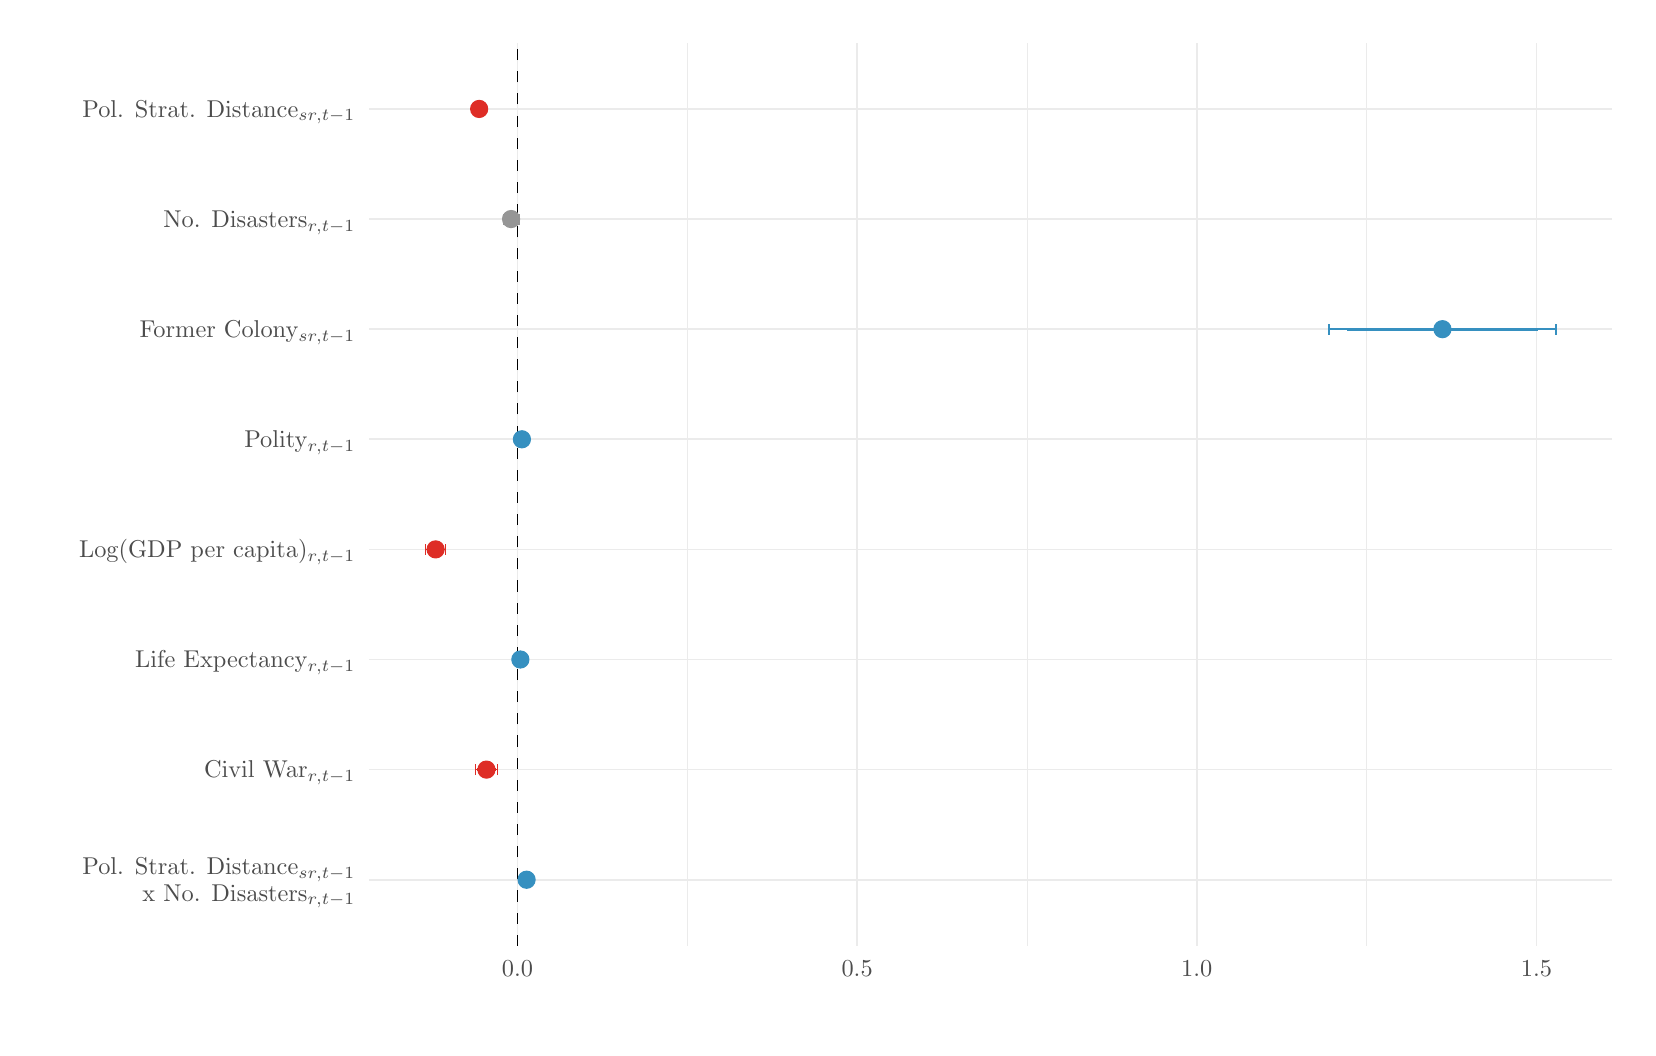
\begin{tikzpicture}[x=1pt,y=1pt]
\definecolor{fillColor}{RGB}{255,255,255}
\path[use as bounding box,fill=fillColor,fill opacity=0.00] (0,0) rectangle (578.16,361.35);
\begin{scope}
\path[clip] (  0.00,  0.00) rectangle (578.16,361.35);
\definecolor{drawColor}{RGB}{255,255,255}
\definecolor{fillColor}{RGB}{255,255,255}

\path[draw=drawColor,line width= 0.6pt,line join=round,line cap=round,fill=fillColor] (  0.00, -0.00) rectangle (578.16,361.35);
\end{scope}
\begin{scope}
\path[clip] (123.37, 29.59) rectangle (572.66,355.85);
\definecolor{fillColor}{RGB}{255,255,255}

\path[fill=fillColor] (123.37, 29.59) rectangle (572.66,355.85);
\definecolor{drawColor}{gray}{0.92}

\path[draw=drawColor,line width= 0.3pt,line join=round] (238.35, 29.59) --
	(238.35,355.85);

\path[draw=drawColor,line width= 0.3pt,line join=round] (361.08, 29.59) --
	(361.08,355.85);

\path[draw=drawColor,line width= 0.3pt,line join=round] (483.81, 29.59) --
	(483.81,355.85);

\path[draw=drawColor,line width= 0.6pt,line join=round] (123.37, 53.46) --
	(572.66, 53.46);

\path[draw=drawColor,line width= 0.6pt,line join=round] (123.37, 93.25) --
	(572.66, 93.25);

\path[draw=drawColor,line width= 0.6pt,line join=round] (123.37,133.04) --
	(572.66,133.04);

\path[draw=drawColor,line width= 0.6pt,line join=round] (123.37,172.82) --
	(572.66,172.82);

\path[draw=drawColor,line width= 0.6pt,line join=round] (123.37,212.61) --
	(572.66,212.61);

\path[draw=drawColor,line width= 0.6pt,line join=round] (123.37,252.40) --
	(572.66,252.40);

\path[draw=drawColor,line width= 0.6pt,line join=round] (123.37,292.19) --
	(572.66,292.19);

\path[draw=drawColor,line width= 0.6pt,line join=round] (123.37,331.98) --
	(572.66,331.98);

\path[draw=drawColor,line width= 0.6pt,line join=round] (176.99, 29.59) --
	(176.99,355.85);

\path[draw=drawColor,line width= 0.6pt,line join=round] (299.72, 29.59) --
	(299.72,355.85);

\path[draw=drawColor,line width= 0.6pt,line join=round] (422.45, 29.59) --
	(422.45,355.85);

\path[draw=drawColor,line width= 0.6pt,line join=round] (545.18, 29.59) --
	(545.18,355.85);
\definecolor{drawColor}{RGB}{222,45,38}

\path[draw=drawColor,draw opacity=0.30,line width= 0.3pt,line join=round] (161.17,331.98) -- (165.12,331.98);
\definecolor{drawColor}{RGB}{150,150,150}

\path[draw=drawColor,draw opacity=0.30,line width= 0.3pt,line join=round] (171.92,292.19) -- (177.44,292.19);
\definecolor{drawColor}{RGB}{54,144,192}

\path[draw=drawColor,draw opacity=0.30,line width= 0.3pt,line join=round] (470.21,252.40) -- (552.24,252.40);

\path[draw=drawColor,draw opacity=0.30,line width= 0.3pt,line join=round] (178.17,212.61) -- (179.00,212.61);
\definecolor{drawColor}{RGB}{222,45,38}

\path[draw=drawColor,draw opacity=0.30,line width= 0.3pt,line join=round] (143.79,172.82) -- (151.04,172.82);
\definecolor{drawColor}{RGB}{54,144,192}

\path[draw=drawColor,draw opacity=0.30,line width= 0.3pt,line join=round] (177.64,133.04) -- (178.41,133.04);
\definecolor{drawColor}{RGB}{222,45,38}

\path[draw=drawColor,draw opacity=0.30,line width= 0.3pt,line join=round] (161.78, 93.25) -- (169.79, 93.25);
\definecolor{drawColor}{RGB}{54,144,192}

\path[draw=drawColor,draw opacity=0.30,line width= 0.3pt,line join=round] (179.51, 53.46) -- (181.04, 53.46);
\definecolor{drawColor}{RGB}{222,45,38}

\path[draw=drawColor,line width= 1.1pt,line join=round] (161.48,331.98) -- (164.81,331.98);
\definecolor{drawColor}{gray}{0.59}

\path[draw=drawColor,line width= 1.1pt,line join=round] (172.36,292.19) -- (176.99,292.19);
\definecolor{drawColor}{RGB}{54,144,192}

\path[draw=drawColor,line width= 1.1pt,line join=round] (476.81,252.40) -- (545.64,252.40);

\path[draw=drawColor,line width= 1.1pt,line join=round] (178.24,212.61) -- (178.94,212.61);
\definecolor{drawColor}{RGB}{222,45,38}

\path[draw=drawColor,line width= 1.1pt,line join=round] (144.37,172.82) -- (150.45,172.82);
\definecolor{drawColor}{RGB}{54,144,192}

\path[draw=drawColor,line width= 1.1pt,line join=round] (177.70,133.04) -- (178.35,133.04);
\definecolor{drawColor}{RGB}{222,45,38}

\path[draw=drawColor,line width= 1.1pt,line join=round] (162.42, 93.25) -- (169.14, 93.25);
\definecolor{drawColor}{RGB}{54,144,192}

\path[draw=drawColor,line width= 1.1pt,line join=round] (179.64, 53.46) -- (180.92, 53.46);
\definecolor{drawColor}{RGB}{0,0,0}

\path[draw=drawColor,line width= 0.6pt,dash pattern=on 4pt off 4pt ,line join=round] (176.99, 29.59) -- (176.99,355.85);
\definecolor{drawColor}{RGB}{222,45,38}
\definecolor{fillColor}{RGB}{222,45,38}

\path[draw=drawColor,line width= 0.4pt,line join=round,line cap=round,fill=fillColor] (163.14,331.98) circle (  3.09);
\definecolor{drawColor}{gray}{0.59}
\definecolor{fillColor}{gray}{0.59}

\path[draw=drawColor,line width= 0.4pt,line join=round,line cap=round,fill=fillColor] (174.68,292.19) circle (  3.09);
\definecolor{drawColor}{RGB}{54,144,192}
\definecolor{fillColor}{RGB}{54,144,192}

\path[draw=drawColor,line width= 0.4pt,line join=round,line cap=round,fill=fillColor] (511.23,252.40) circle (  3.09);

\path[draw=drawColor,line width= 0.4pt,line join=round,line cap=round,fill=fillColor] (178.59,212.61) circle (  3.09);
\definecolor{drawColor}{RGB}{222,45,38}
\definecolor{fillColor}{RGB}{222,45,38}

\path[draw=drawColor,line width= 0.4pt,line join=round,line cap=round,fill=fillColor] (147.41,172.82) circle (  3.09);
\definecolor{drawColor}{RGB}{54,144,192}
\definecolor{fillColor}{RGB}{54,144,192}

\path[draw=drawColor,line width= 0.4pt,line join=round,line cap=round,fill=fillColor] (178.03,133.04) circle (  3.09);
\definecolor{drawColor}{RGB}{222,45,38}
\definecolor{fillColor}{RGB}{222,45,38}

\path[draw=drawColor,line width= 0.4pt,line join=round,line cap=round,fill=fillColor] (165.78, 93.25) circle (  3.09);
\definecolor{drawColor}{RGB}{54,144,192}
\definecolor{fillColor}{RGB}{54,144,192}

\path[draw=drawColor,line width= 0.4pt,line join=round,line cap=round,fill=fillColor] (180.28, 53.46) circle (  3.09);
\definecolor{drawColor}{RGB}{222,45,38}

\path[draw=drawColor,line width= 0.6pt,line join=round] (165.12,329.99) --
	(165.12,333.97);

\path[draw=drawColor,line width= 0.6pt,line join=round] (165.12,331.98) --
	(161.17,331.98);

\path[draw=drawColor,line width= 0.6pt,line join=round] (161.17,329.99) --
	(161.17,333.97);
\definecolor{drawColor}{gray}{0.59}

\path[draw=drawColor,line width= 0.6pt,line join=round] (177.44,290.20) --
	(177.44,294.18);

\path[draw=drawColor,line width= 0.6pt,line join=round] (177.44,292.19) --
	(171.92,292.19);

\path[draw=drawColor,line width= 0.6pt,line join=round] (171.92,290.20) --
	(171.92,294.18);
\definecolor{drawColor}{RGB}{54,144,192}

\path[draw=drawColor,line width= 0.6pt,line join=round] (552.24,250.41) --
	(552.24,254.39);

\path[draw=drawColor,line width= 0.6pt,line join=round] (552.24,252.40) --
	(470.21,252.40);

\path[draw=drawColor,line width= 0.6pt,line join=round] (470.21,250.41) --
	(470.21,254.39);

\path[draw=drawColor,line width= 0.6pt,line join=round] (179.00,210.62) --
	(179.00,214.60);

\path[draw=drawColor,line width= 0.6pt,line join=round] (179.00,212.61) --
	(178.17,212.61);

\path[draw=drawColor,line width= 0.6pt,line join=round] (178.17,210.62) --
	(178.17,214.60);
\definecolor{drawColor}{RGB}{222,45,38}

\path[draw=drawColor,line width= 0.6pt,line join=round] (151.04,170.83) --
	(151.04,174.81);

\path[draw=drawColor,line width= 0.6pt,line join=round] (151.04,172.82) --
	(143.79,172.82);

\path[draw=drawColor,line width= 0.6pt,line join=round] (143.79,170.83) --
	(143.79,174.81);
\definecolor{drawColor}{RGB}{54,144,192}

\path[draw=drawColor,line width= 0.6pt,line join=round] (178.41,131.05) --
	(178.41,135.03);

\path[draw=drawColor,line width= 0.6pt,line join=round] (178.41,133.04) --
	(177.64,133.04);

\path[draw=drawColor,line width= 0.6pt,line join=round] (177.64,131.05) --
	(177.64,135.03);
\definecolor{drawColor}{RGB}{222,45,38}

\path[draw=drawColor,line width= 0.6pt,line join=round] (169.79, 91.26) --
	(169.79, 95.24);

\path[draw=drawColor,line width= 0.6pt,line join=round] (169.79, 93.25) --
	(161.78, 93.25);

\path[draw=drawColor,line width= 0.6pt,line join=round] (161.78, 91.26) --
	(161.78, 95.24);
\definecolor{drawColor}{RGB}{54,144,192}

\path[draw=drawColor,line width= 0.6pt,line join=round] (181.04, 51.47) --
	(181.04, 55.45);

\path[draw=drawColor,line width= 0.6pt,line join=round] (181.04, 53.46) --
	(179.51, 53.46);

\path[draw=drawColor,line width= 0.6pt,line join=round] (179.51, 51.47) --
	(179.51, 55.45);
\end{scope}
\begin{scope}
\path[clip] (  0.00,  0.00) rectangle (578.16,361.35);
\definecolor{drawColor}{gray}{0.30}

\node[text=drawColor,anchor=base east,inner sep=0pt, outer sep=0pt, scale=  0.88] at (118.42, 55.18) {Pol. Strat. Distance$_{sr,t-1}$ };

\node[text=drawColor,anchor=base east,inner sep=0pt, outer sep=0pt, scale=  0.88] at (118.42, 45.68) { x No. Disasters$_{r,t-1}$};

\node[text=drawColor,anchor=base east,inner sep=0pt, outer sep=0pt, scale=  0.88] at (118.42, 90.22) {Civil War$_{r,t-1}$};

\node[text=drawColor,anchor=base east,inner sep=0pt, outer sep=0pt, scale=  0.88] at (118.42,130.01) {Life Expectancy$_{r,t-1}$};

\node[text=drawColor,anchor=base east,inner sep=0pt, outer sep=0pt, scale=  0.88] at (118.42,169.79) {Log(GDP per capita)$_{r,t-1}$};

\node[text=drawColor,anchor=base east,inner sep=0pt, outer sep=0pt, scale=  0.88] at (118.42,209.58) {Polity$_{r,t-1}$};

\node[text=drawColor,anchor=base east,inner sep=0pt, outer sep=0pt, scale=  0.88] at (118.42,249.37) {Former Colony$_{sr,t-1}$};

\node[text=drawColor,anchor=base east,inner sep=0pt, outer sep=0pt, scale=  0.88] at (118.42,289.16) {No. Disasters$_{r,t-1}$};

\node[text=drawColor,anchor=base east,inner sep=0pt, outer sep=0pt, scale=  0.88] at (118.42,328.95) {Pol. Strat. Distance$_{sr,t-1}$};
\end{scope}
\begin{scope}
\path[clip] (  0.00,  0.00) rectangle (578.16,361.35);
\definecolor{drawColor}{gray}{0.30}

\node[text=drawColor,anchor=base,inner sep=0pt, outer sep=0pt, scale=  0.88] at (176.99, 18.58) {0.0};

\node[text=drawColor,anchor=base,inner sep=0pt, outer sep=0pt, scale=  0.88] at (299.72, 18.58) {0.5};

\node[text=drawColor,anchor=base,inner sep=0pt, outer sep=0pt, scale=  0.88] at (422.45, 18.58) {1.0};

\node[text=drawColor,anchor=base,inner sep=0pt, outer sep=0pt, scale=  0.88] at (545.18, 18.58) {1.5};
\end{scope}
\end{tikzpicture}
